
\chapter{Evolution du système}\label{ch:produit}

Le développement d'un prototype du système, réalisé dans le cadre de ce travail de Bachelor, a permis de montrer que le concept dans son ensemble est fonctionnel, cependant encore beaucoup de travail reste à réaliser. Ce chapitre propose quelques étapes afin de faire évoluer le prototype vers un produit à part entière.

\section{Centralisation des données}

Dès que l'on souhaite utiliser plus d'une passerelle, il devient indispensable de centraliser la base de données sur un serveur accessible depuis internet. En effet, dans ce cas on ne peut plus se contenter de stocker toutes les données sur la passerelle.

Pour ce faire, il faut donc héberger la base de données sur un serveur. Afin que toutes les passerelles puissent ensuite accéder à la base, il est nécessaire d'équiper chaque passerelle d'un moyen de connexion, par le réseau GSM mobile par exemple. Le logiciel du serveur d'application doit aussi être modifié afin de prendre en compte ce changement. De plus il faudra prendre gare à la gestion des données dupliquées. En effet, il est tout à fait possible que deux passerelles différentes reçoivent le même paquet. Dans un tel cas il faut donc vérifier que les données ne sont pas déjà enregistrées dans la base de données avant de les sauvegarder.

Une fois ces modifications apportées au système, les passerelles sont en mesure de stocker les données en provenance des capteurs sur une base de données centralisée.

\section{Concentrateur multi-canaux}

Lors du développement du projet, pour des raisons de coût, il a été décidé d'utiliser un concentrateur simple-canal dont le principe est que le capteur et la passerelle doivent utiliser un seul et même canal pour le transfert des données. Pour un prototype, cette solution est adéquate, cependant cette approche n'est pas optimale pour une évolution du système.

Une passerelle multi-canaux est indispensable dans une optique produit. En effet, pour diminuer l’influence des interférences, les capteurs changent le canal sur lequel les paquets sont transmis, ce qui apporte une robustesse supplémentaire au système. Cette technique requiert d'avoir des passerelles munies de concentrateurs multi-canaux pour pouvoir fonctionner.

\section{Création d'une API web moderne}

Afin de rendre l'accès aux données mieux structuré et plus robuste, la conception d'une API web moderne, de type REST, est indispensable. L'application mobile, pour des raisons de simplifications, accède directement au données en envoyant des requêtes SQL au serveur qui héberge la base de données.

Le fait d'utiliser un tel type d'API permet de déplacer la majeure partie du travail de calcul du téléphone mobile au serveur en charge de l'interface. Cela a l'avantage d'augmenter la durée de vie de la batterie des téléphones qui exécutent l'application, la gestion entière de la construction des requêtes et de la connexion étant dévolue au téléphone mobile. Dans le cas d'une API REST, c'est le serveur qui fait l’entier du travail, le téléphone mobile accédant en essence uniquement au contenu de page web. Un autre aspect intéressant de cette technique est qu’elle diminue la quantité de données transférées entre le serveur et le téléphone, et donc la bande passante nécessaire, ce qui peut être appréciable pour les utilisateurs ayant une quantité de données limitée.

Un autre avantage de poids est le fait que de cette façon le design de la base de données et celui de l'application mobile ne sont plus couplés. En effet, dans le cas où les requêtes sont exécutées par le téléphone mobile, la structure des tables doit lui être connue, ce qui fait que tout changement à la base de données engendre des modifications également dans l'application mobile.

\section{Augmentation du nombre de capteurs et de passerelles}

Un aspect qui semble être évident est d'augmenter le nombre de capteurs et de passerelles utilisés en parallèle. En effet, puisque le travail de Bachelor a été développé pour l'utilisation d'un seul capteur et d'une seule passerelle, beaucoup de cas d'utilisation n'ont pas pu être testés, comme par exemple la charge additionnelle que plusieurs capteurs ajouteraient au système et qui pourrait rendre le système inutilisable.

\section{Utilisation de LoRaWAN}

Afin de rendre le système plus robuste et performant, l'utilisation de la couche MAC LoRaWAN peut s’avérer utile. Le chiffrement des données entre les capteurs et le serveur réseau augmente la sécurité du système et le fait que LoRaWAN utilise un mécanisme de connexion au réseau permet également une meilleure gestion d'un grand nombre de capteurs en même temps. En plus de cela, la gestion de l'optimisation du débit de transfert des nœuds par le serveur réseau permet d'améliorer le rendement du système dans son entièreté.

Un avantage de l'utilisation de LoRWAN réside dans le fait qu'il devient alors possible pour les capteurs de transférer des données en passant par une passerelle faisant partie d'un réseau privé, comme celui de Swisscom par exemple. Le fait d'augmenter le nombre de passerelle avec lesquelles les capteurs sont en mesure de transférer leurs données ajoute encore à la robustesse du système. Cette solution permet également d'utiliser des serveurs d'application de communautés existantes comme par exemple TheThingsNetwork. Le protocole est alors entièrement géré par ce serveur, il reste ensuite à mettre en place un serveur d'application qui permet la gestion et l'exploitation des données reçues depuis les capteurs.

La figure \ref{fig:sys_infra_evol} montre l'infrastructure du système avec utilisation de LoRaWAN.

\begin{figure}[tb]
\centering 
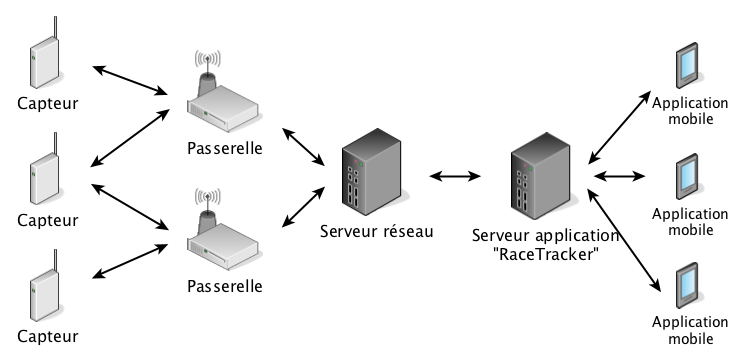
\includegraphics[width=0.8\columnwidth]{systeme_evolution.png} 
\caption{Infrastructure du système avec utilisation de LoRaWAN}
\label{fig:sys_infra_evol}
\end{figure}

\section{D'avantage d'interactivité dans l'application mobile}

Un des aspects du système qui peut également être développé davantage est l'application mobile. En effet, la version développée pendant ce projet se concentre sur l’essentiel. Dans la mesure où le but du système est d'impliquer davantage les spectateurs aux courses, on pourrait envisager des fonctionnalités permettant aux utilisateurs d'échanger des opinions par le biais d'un chat, ou de partager des photos des participants prises le long du parcours. 

Une autre idée pourrait consister à ajouter un système, piloté par les organisateurs de la course, qui pourrait leur permettre de commenter en direct la compétition avec des messages spéciaux pour attirer l'œil des spectateurs sur les moments clefs. Le système pourrait également donner des informations générales, par exemple sur une certaines distance atteinte par la tête de la course ou un dénivelé important gravi par les coureurs. L'intégration de Twitter dans l'application est également une possibilité permettant aux spectateurs de partager des discussions entre eux.

Enfin, l'analyse des données pourrait être davantage mise à l'avant, avec par exemple la possibilité de consulter divers graphiques montrant l'évolution de la vitesse et du rythme cardiaque d'une sélection d'athlète afin de pouvoir comparer leurs performances.

\section{Configuration précise du système}

Le système est dépendant de beaucoup de paramètres différents. Pour son évolution, il serait important de pouvoir faire de nombreux tests supplémentaires en essayant de trouver les valeurs optimales de ses paramètres. Le facteur d'étalement ainsi que la puissance du signal sont deux éléments cruciaux pour le système qui déterminent à la fois la qualité de la transmission des données et également la fiabilité du système dans son ensemble. Si les données ne sont pas en mesure d'être captées par les passerelles, le système ne fonctionne tout simplement pas. Afin d'arriver à trouver la configuration la mieux adaptée, il faut essayer le maximum de combinaisons dans des conditions différentes, dans un espace dégagé mais également dans des endroits accidentés comme en montagne par exemple, avec une puissance maximale mais également tenter de trouver la puissance minimale à laquelle le système est toujours capable de fonctionner. Au vu du nombre élevé des possibilités disponibles et du temps nécessaire à les tester, ces activités ne peuvent pas toutes être réalisées durant le travail de Bachelor.